\documentclass[12pt]{article}
\usepackage{graphicx}
\usepackage {color}
\usepackage{pdfpages}
\usepackage{float}
\usepackage{changebar}
\usepackage{enumitem,amssymb}
\renewcommand{\familydefault}{\sfdefault}
\usepackage[margin=1.2in]{geometry}
\usepackage{graphicx}
\usepackage{wrapfig}
\usepackage[super]{cite}
\usepackage{subcaption}
\usepackage[table]{xcolor}
\usepackage{amsmath}
\usepackage[sort, numbers]{natbib}
\usepackage{multirow}
\usepackage{tabularx}
\usepackage{siunitx}

%%%%%%%%%%%%Defining the margins %%%%%%%%%%%%%%%%%%%%%
\textheight 9.in
\textwidth 6.5in
\topmargin -.5in
\oddsidemargin 0in
\setlength{\parskip}{\smallskipamount}

%%%%%%%%%%%%%%Specific Commands %%%%%%%%%%%%%%%%%%
\newcommand{\eg}{{\em e.g.,}}
\newcommand{\ie}{{\em i.e.,}}
\newcommand{\etc}{{\em etc.,}}
\newcommand{\etal}{{\em et al.}}
\newcommand{\degrees}{{$^{\circ}$}}
\newcommand{\fig}[1]{\textbf{Figure #1}}
\DeclareMathOperator*{\argmin}{argmin}
%%%%%%%%%%%%%%%%%%%%%%%%%%%% Setting to control figure placement
% These determine the rules used to place floating objects like figures 
% They are only guides, but read the manual to see the effect of each.
\renewcommand{\topfraction}{.9}
\renewcommand{\bottomfraction}{.9}
\renewcommand{\textfraction}{.1}
\renewcommand{\familydefault}{\sfdefault} %setting the san serif font

%%%%%%%%%%%%%%%%%%%%%%%% Line spacing
% Use the following command for ``double'' spacing
%\setlength{\baselineskip}{1.2\baselineskip}
% and this one for an acceptable NIH spacing of 6lpi based on 11pt
%\setlength{\baselineskip}{.9\baselineskip}
% The baselineskip does not appear to work when we include a maketitle
% command in the main file.  Something there must set the line spacing
% If we use this next command, then things seem to work.
\renewcommand{\baselinestretch}{.9}
\newcommand{\rpm}{\raisebox{.2ex}{$\scriptstyle\pm$}}
\setcounter{secnumdepth}{0} %make no numbers but have a table of contents


\begin{document}

\title{Term Project: Optimization of Reconstruction}
\author{Jake Bergquist, u6010393 }
\maketitle

\section{Introduction}
Work done in our labs has shown that an incomplete sampling of the epicardial
potentials during our typical experimental preparations creates significant error
during computational modeling of the heart.\cite{RSM:Tat2018b} Many experimental preparations such as those used in our labs as well as those of collaborators utilize these epicardial sock electrode arrays that only provide partial coverage of the cardiac source.\cite{RSM:Bur2018b,Zenger2019,RSM:Goo2018,RSM:Bea2015a} In such
cases, we must aproximate the missing data on the atria from the signals we do recover on the ventricles. A
common approach that we have used in the past is to approximate the missing signals by interpolating from the
measured data often using a surface Laplacian approach, however, it is
unclear if interpolation approaches are able to reconstruct the missing
atrial signals in a scenario in which only ventricular signals are
measured.\cite{Huiskamp1991}

To address the difficulties we encounter with this reconstruction we developed an experimental setup where we utilize a rigid peri-cardiac cage that forms a closed surface of recording electrodes around the cardiac source. This cage is constructed such that each electrode has equal solid angle to the center of the cage and should capture the entire cardiac surface.

Before addressing the reconstruction techniques I need to employ on the epicardial sock electrode array I wanted to work with a more simple case in which only the cardiac cage was considered. I divided the cage into a ventricular (lower) segment and an segment. I then formulated two optimization problems in order to address the reconstruction of the upper atrial portion of the cage using the lower ventricular signals. The key difference between the two methods was one utilized only the time signals while the other optimized a term for the time derivative of the signals. I tested these methods across three beat morphologies. I found good agreement of the reconstructed signals when compared to the measured. By contrast the Laplacian interpolation over the upper region performed poorer in all cases, specifically with more complicated beat morphologies resulting int he poorest Laplacian reconstruction.

I then formulated an optimization of the reconstruction of the atrial signals from the ventricular signals by informing the reconstruction using the cage potentials. Utilizing the boundary element formulation I can solve laplaces equation through the volume between the epicardial sock and the cage to calculate what the potential distribution should be on the cage given a certain sock potential distribution. This formulation however requires a closed inner source surface, hence why we need to recreate the atrial potentials. By minimizing the difference between these forward computed potentials and the measured cage potentials over an interpolation/reconstruction matrix that gives us our atrial signals we can optimize this reconstruction matrix.

\section{Methods}

The pericardiac cage utilized is shown in Figure~\ref{Fig:Cag}. As can be seen the cage is made up of many (256) recording electrode positions held in place by a 3D printed frame. The potential distribution (in milivolts) at a specific time instance during a heartbeat is shown the left in Figure~\ref{Fig:Cag} demonstrating that the cage is able to record simultaneous electrical recordings from the entire cage surface. This cage was divided in a manner similar to the scenario seen in experimental situations where the atrial region (top) is considered missing data that the ventricular (bottom) region must be used to reconstruct. The atrial region ($C_A$) is comprised of the top quarter of the cage (the top 4 rings) and the ventricular region ($C_V$) is comprised of the remaining three quarters of the cage. I then designed a basic optimization approach to calculate a matrix, $D$ that maps $C_V$ to $C_A$. By minimizing Equation~\ref{EQ:Opt1} over $D$ we obtain an optimal $D$.

\begin{figure}[h]
	% \centering
	\includegraphics[width=0.9\textwidth]{Figures/CageFigure.png}
	\caption{The Utah Pericardiac Cage (UPC)[. The UPC] is a 3D printed
		structure that has mounting holes for 256 recording
		electrodes; one such electrode location is circled in red. The electrode locations connect to form
		triangles, all of which have approximately equal solid
		angles with respect to the centroid of the cage. The two halves of
		the UPC are closed around the isolated heart and both the UPC and
		heart are immersed in a torso tank filled with
		electrolyte. The recorded signals can be mapped onto a digitized
		geometry of the electrode locations. Colors here represent the
		potential distribution at a time instant 50\% into the QRS of a sinus
		beat.}
	\label{Fig:Cag}
\end{figure}



\begin{equation}
\argmin_{D} ||DC_V - C_A||^2
\label{EQ:Opt1}
\end{equation}

\begin{equation}
(DC_V - C_A)^T(DC_V - C_A)
\label{EQ:Opt1_1}
\end{equation}

\begin{equation}
C_V^TD^TDC_V  - 2C_V^TD^TC_A - C_A^TC_A
\label{EQ:Opt1_2}
\end{equation}

\begin{equation}
D(2C_VC_V^T) - 2C_AC_V^T - 0 = 0
\label{EQ:Opt1_3}
\end{equation}

\begin{equation}
D = C_AC_V^T(C_VC_V^T)^{-1}
\label{EQ:Opt1_4}
\end{equation}

\begin{equation}
D^{I+1} = D^I + \epsilon(2D^NC_VC_V^T - 2C_AC_V^T)
\label{EQ:Opt1_5}
\end{equation}

We can solve this optimization problem by expanding Equation~\ref{EQ:Opt1} into Equation~\ref{EQ:Opt1_1} which can be epanded further to give Equation~\ref{EQ:Opt1_2}. Taking the derivative with respect to $D$ and setting this equal to zero gives Equation~\ref{EQ:Opt1_3}. From here we can either solve using gradient descent (Equation~\ref{EQ:Opt1_5}) or by simply solving for the optimal $D$ as in Equation~\ref{EQ:Opt1_4}. The second optimization formulation takes into account an additional parameter. Because $C_V$ and $C_A$ are comprised of time signals it would make sense to include information about the time derivative of these signals in the form of another interpolation matrix that weights these time derivative terms. We see this in Equation~\ref{EQ:Opt2} where not only do we weight the time signals ($E$) but also we add a mapping matrix, $F$, that weights the derivative of $C_V$ with respect to time ($C'_v$).

\begin{equation}
\argmin_{E,F} ||EC_V + FC'_V - C_A||^2
\label{EQ:Opt2}
\end{equation}

\begin{equation}
C_V^TE^TEC_V + 2C_V^TE^TFC'_V - 2C_V^TE^TC_A + C'_V^TF^TFC'_V - 2C'_V^TF^TC_A + C_A^TC_A
\label{EQ:Opt2_1}
\end{equation}

\begin{equation}

\label{EQ:Opt2_2}
\end{equation}

\section{Results}


\begin{table}[htbp]
	\centering
	\caption{\label{tab:err} Numerical results from the three reconstruction scenarios. Maximum, mean, and standard deviation or error displayed in mV.}
	%\centering
	\begin{tabular}{|lr|r|r|r|} \hline
		&&Ventricular&Sinus&Atrial\\
		Method&&Paced&&Paced\\
		&&(mV)&(mV)&(mV)\\
		\hline
		\multirow{3}{*}{Opt. 1}
		&Max Err.&0.35&0.16&1.0\\
		&Mean Err.&0.011&0.011&0.017\\
		&STD&\rpm{}0.018&\rpm{}0.013&\rpm{}0.039\\
		\hline
		\multirow{3}{*}{Opt. 2}
		&Max Err.&0.41&0.21&1.0\\
		&Mean Err.&0.013&0.015&0.017\\
		&STD&\rpm{}0.021&\rpm{}0.016&\rpm{}0.040\\
		\hline
		\multirow{3}{*}{Laplacian}
		&Max Err.&1.5&2.6&11\\
		&Mean Err.&0.071&0.11&0.10\\
		&STD&\rpm{}0.11&\rpm{}0.18&\rpm{}0.38\\
		\hline
		
	\end{tabular}
\end{table}

The potential distributions of the Laplacian interpolated and the optimized
reconstructed signals varied greatly. The two optimized reconstructions
resulted in similar distributions that agreed with the measured
distributions. The Laplacian interpolated signals showed reasonable
agreement with the measured signals for the ventricular paced beat
morphologies. However, there was striking disagreement between the
Laplacian interpolated and measured signals for both the sinus and atrial
paced morphologies. The potential distributions for each beat
at 50\% into the QRS complex are displayed in Figure~\ref{Fig:Res}.


\begin{figure}[h]
	% \centering
	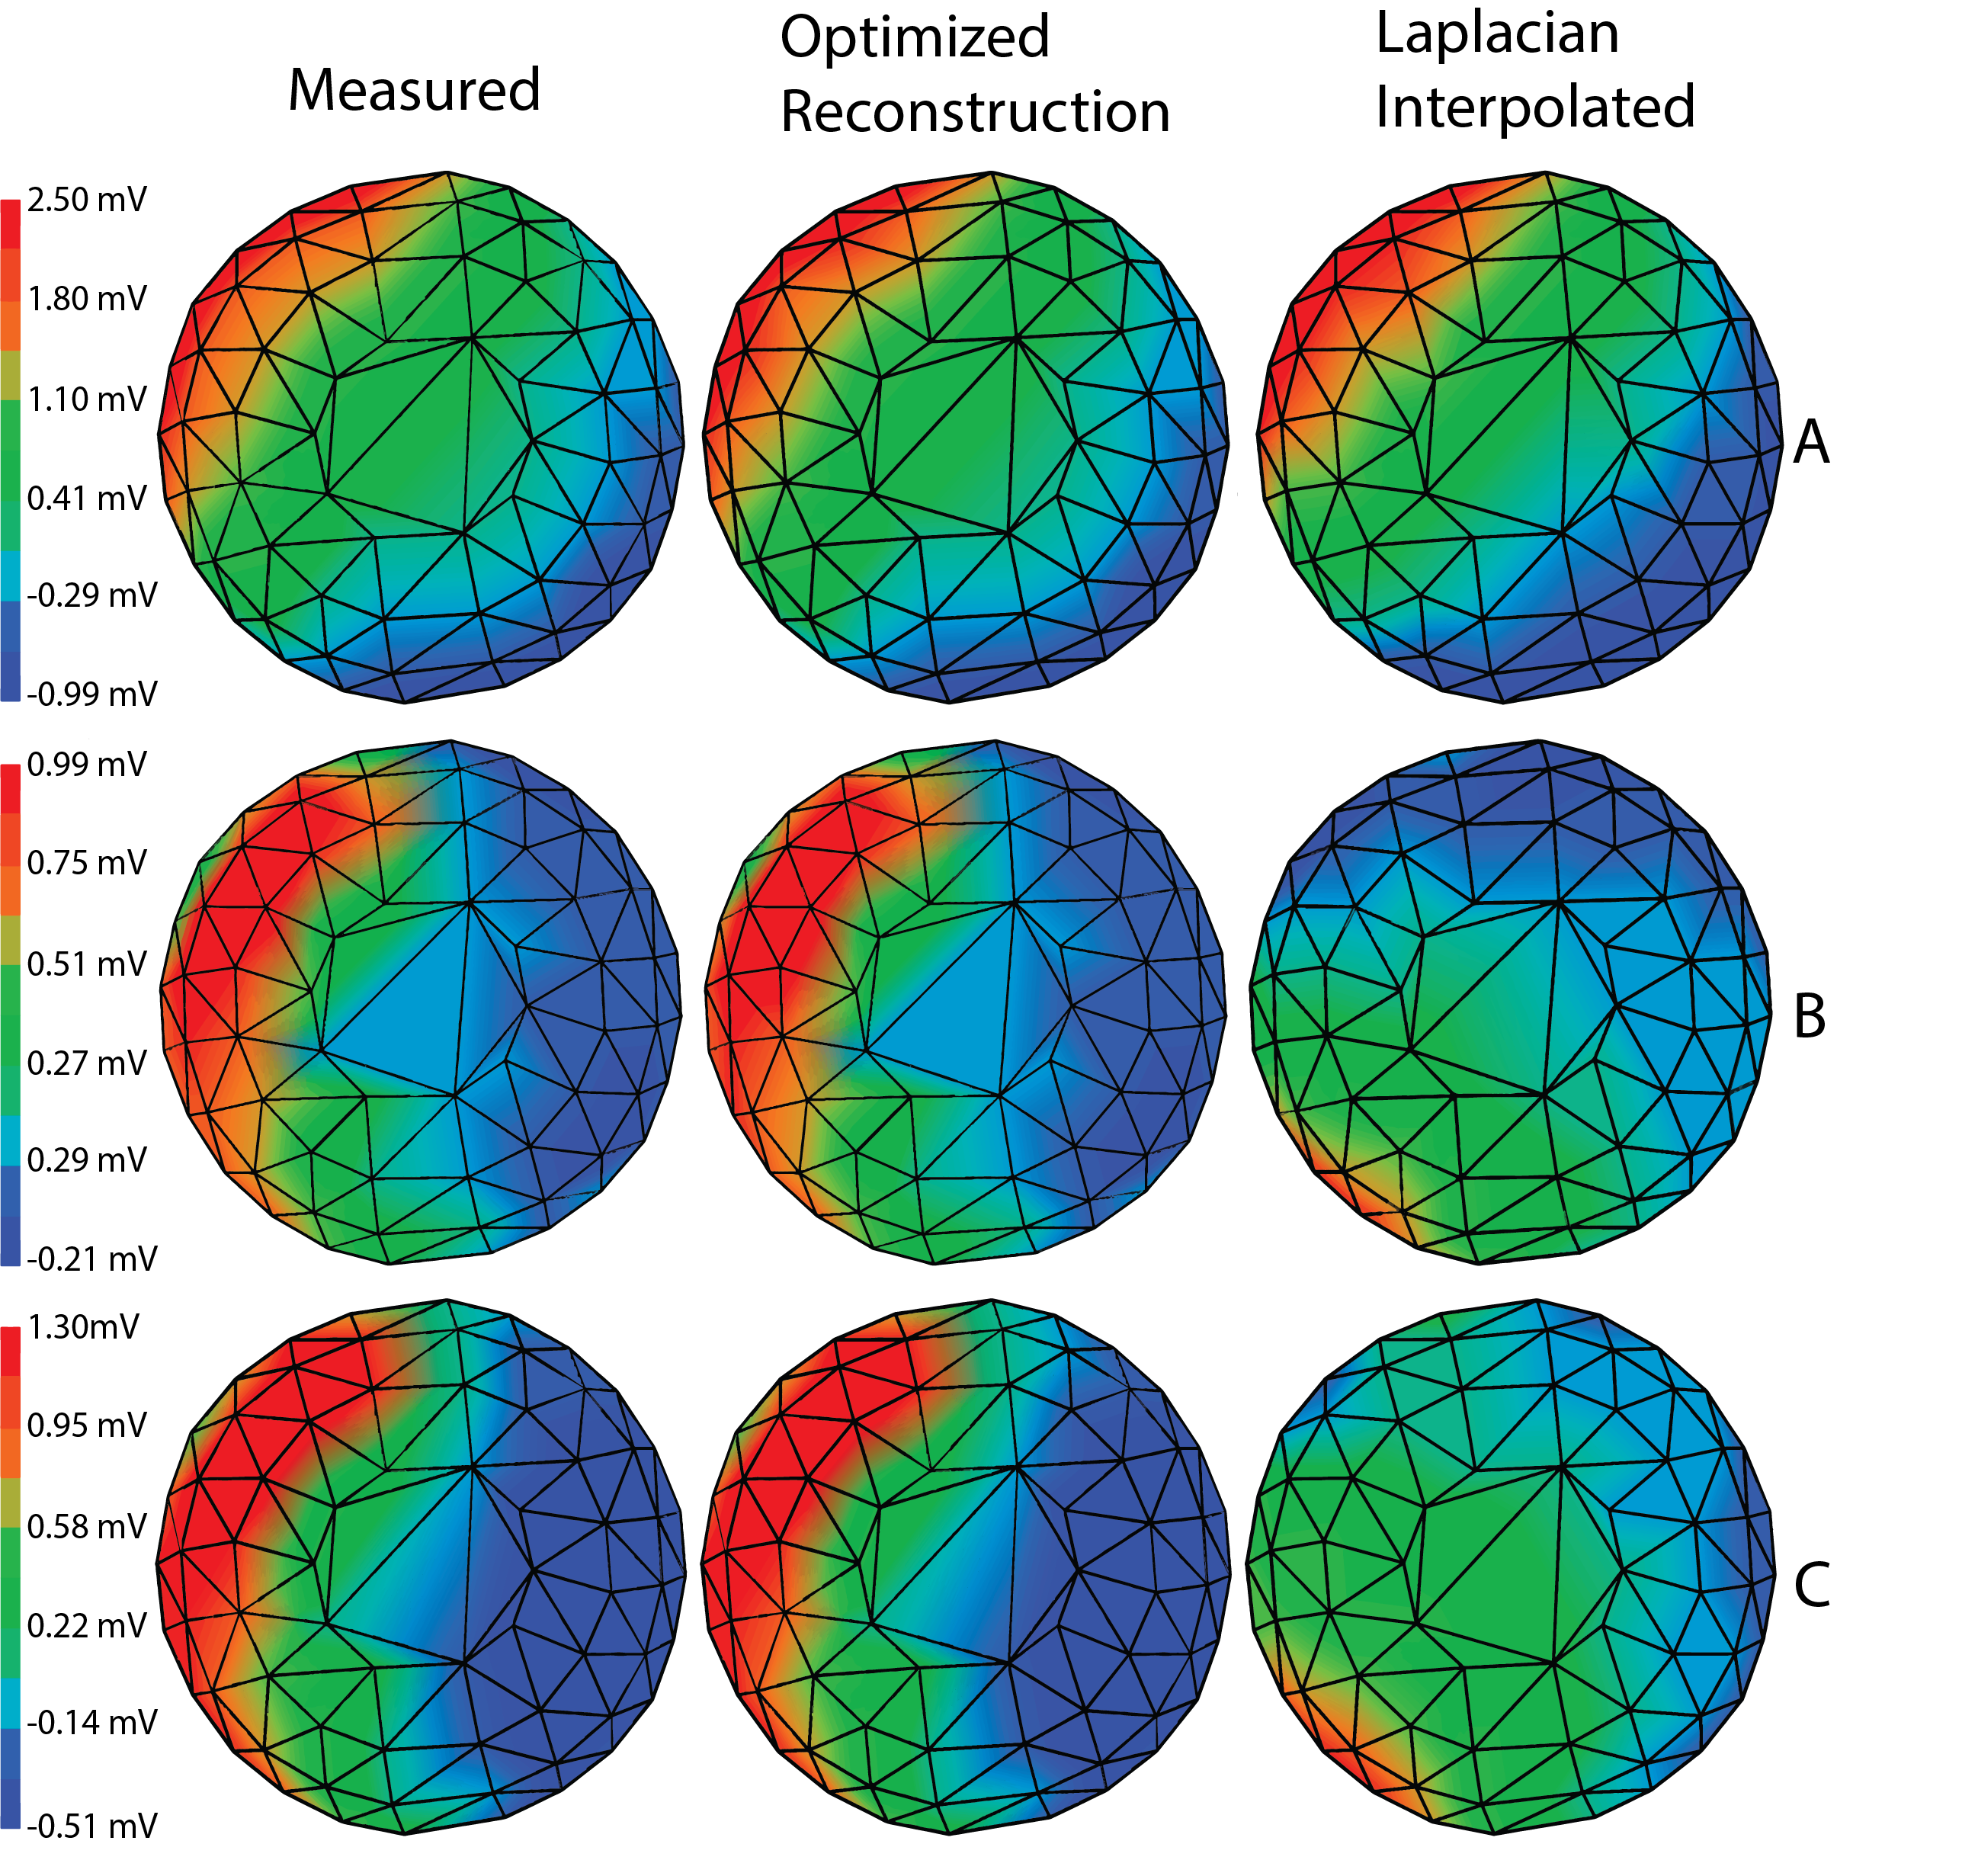
\includegraphics[width=0.9\textwidth]{Figures/Figure1.png}
	\caption{Potentials on the basal subset of the cage for each
		reconstruction method across three beat morphologies. The time point
		displayed for each case is 50\% into the QRS complex. The measured
		column shows the signals measured from the cage. The optimized
		reconstruction column shows potentials from the Opt. 1 method. The
		Laplacian Interpolation column shows the potentials from the spatial
		Laplacian interpolation. Row A shows a ventricular paced beat. Row B
		shows sinus beat. Row C shows an atrial paced beat.}
	\label{Fig:Res}
\end{figure}


\section{Discussion}

%%%%%%%%%%%%%%%%%% Correct Bibliography Style

\bibliography{library,biglit,strings}
\bibliographystyle{IEEEtran}


\end{document}








